\documentclass[14pt, a4paper]{article}

\usepackage[utf8]{inputenc}
\usepackage[russian]{babel}
\usepackage[T2A]{fontenc}
\usepackage{amsmath}
\usepackage{indentfirst}
\usepackage[final]{graphicx}
\usepackage{floatflt}

\graphicspath{{images/}}
\usepackage{geometry}
\geometry{left=2cm}% левое поле
\geometry{right=1.5cm}% правое поле
\geometry{top=1cm}% верхнее поле
\geometry{bottom=2cm}% нижнее поле

\renewcommand{\theenumi}{\arabic{enumi}}% Меняем везде перечисления на цифра.цифра
\renewcommand{\labelenumi}{\arabic{enumi}}% Меняем везде перечисления на цифра.цифра
\renewcommand{\theenumii}{.\arabic{enumii}}% Меняем везде перечисления на цифра.цифра
\renewcommand{\labelenumii}{\arabic{enumi}.\arabic{enumii}.}% Меняем везде перечисления на цифра.цифра
\renewcommand{\theenumiii}{.\arabic{enumiii}}% Меняем везде перечисления на цифра.цифра
\renewcommand{\labelenumiii}{\arabic{enumi}.\arabic{enumii}.\arabic{enumiii}.}% Меняем везде перечисления на цифра.цифра

\begin{document}
	\begin{titlepage}
	\fontsize{16}{20pt}\selectfont
	\newpage
	
	\begin{center}
		МОСКОВСКИЙ ГОСУДАРСТВЕННЫЙ УНИВЕРСИТЕТ ИМЕНИ М.В.ЛОМОНОСОВА
	\end{center}
	\vspace{2em}
	
	\begin{center}
ФИЗИЧЕСКИЙ ФАКУЛЬТЕТ
	\end{center}
	\vspace{1em}
	\begin{center}
		КАФЕДРА ФИЗИКИ КОСМОСА
	\end{center}
	\vspace{2em}
	
	\begin{center}
КУРСОВАЯ РАБОТА
	\end{center}
		
	\vspace{2em}
	\begin{center}
		Черенковские детекторы в спектрометрии электронов в диапазоне 1--10 МэВ
	\end{center}
	\vspace{8em}
	
	\newbox{\lbox}
	\savebox{\lbox}{\hbox{Илья Александрович Рубинштейн}}
	\newlength{\maxl}
	\setlength{\maxl}{\wd\lbox plus 1ex}
	\hfill\parbox{11cm}{
		\hspace*{2cm}\hspace*{-4cm}Студент:\hfill\hbox to\maxl{ Александр Юрьевич Разумов\hfill}\\
		\hspace*{2cm}\hspace*{-4cm}Преподаватель: \hfill\hbox to\maxl{Илья Александрович Рубинштейн}\\
		\\
		\hspace*{2cm}\hspace*{-4cm}Группа: \hfill\hbox to\maxl{205}\\
	}
	\vspace{\fill}
	
	\begin{center}
		Москва \\2018
	\end{center}
	
	
\end{titlepage}% это титульный лист
	\tableofcontents
	\begin{Kur-Description}
	\fontsize{16}{14pt}\selectfont
	\newpage
	
	\part{Введение}
	\label{sec:part}
\section{Введение}
\label{sec:section}
\subsection{Цель работы}
\label{sec:subsection}
 Изучение принципов функционирования черенковских детекторов, их типы, характеристики, области применения. Отдельное внимание уделяется характеристикам прибора, таким как угловое, энергетическое, скоростное и временное разрешение для регистрации электронов с энергиями из диапазона 1 -- 10 МэВ. 

\subsection{Актуальность} 
\label{sec:subsection}
Черенковские детекторы обеспечили возможность постановки и проведения многочисленных экспериментов различных физических направлений, диапазон которых чрезвычайно широк. Они используются при регистрации космических лучей экстремальных энергий (КЛЭЭ). Детекторы занимают особое место в нейтринной астрономии. Сегодня работают нейтринные телескопы на основе черенковских счётчиков (НТ-200, ANTARES, NESTOR) для регистрации нейтрино сверхвысоких энергий. Они позволяют вести спектрометрию частиц, приходящих из космоса. В частности, из спектров электронов определяют их происхождение а также процессы, происходящие на Солнце.

\subsection{Основные этапы работы}
\label{sec:subsection}
Непосредственно из цели вытекают задачи:
\begin{enumerate}
	\item Изучить механизм возникновения черенковского излучения, его свойства, способы его применения;
	\item Классифицировать черенковские счётчики, проанализировать их характеристики, внутреннее устройство;
	\item Собрать информацию о применении черенковских детекторов в физике частиц;
	\item Рассчитать разрешение для дифференциального черенковского счётчика. 
\end{enumerate}
\end{Kur-Description}% это описание
	\begin{main}
	\def\dd#1#2{\frac{d#1}{d#2}}
	\fontsize{16}{14pt}\selectfont
	\part{Основная часть}	
	\label{sec:part}
	
	\section{Явление черенковского излучения}
	\label{sec:section}
	
	\subsection{История открытия}
	\label{sec:subsection}
	В~1934~г. Павел Алексеевич Черенков, аспирант С.И.~Вавилова, обнаружил неизвестное ранее голубое свечение прозрачных жидкостей под действием $\gamma$-излучения. 
	В его эксперименте в качестве последних выступали растворы солей урана, а источником $\gamma$-квантов служил радиоактивный препарат, содержащий несколько грамм радия.
	 Анализируя исследованные П.А.~Черенковым свойства этого излучения, С.И.~Вавилов предположил, что открытое излучение связано с движением в среде заряженной частицы. 
	 Механизм нового эффекта --- возникновение светового излучения при движении заряженной частицы со скоростью $v$, превышающей фазовую скорость света $c/n$ в веществе с показателем преломления $n$ --- был выяснен в работе И.Е.~Тамма и И.М.~Франка (1937 г.), которая содержала и его количественную теорию.
	 В эксперименте Черенкова гамма-излучение выбивает электроны из атомов среды, те~приобретают скорости, превышающие скорость света в среде, и возникало явление, подобное ударной волне, производимой в атмосфере сверхзвуковым самолётом.
	 Это выдающееся открытие получило признание мирового физического сообщества, и~в~1960~г. его авторы (П.А.~Черенков, И.Е.~Тамм, И.М.~Франк) стали лауреатами Нобелевской премии.
	 В результате трудных и детальных исследований Черенкову удалось установить ряд свойств получаемого излучения, которые противоречили свойствам люминесценции, к которой изначально его относили:
	 \begin{itemize}
	 	\item Интенсивность и спектр излучения почти не зависят от типа вещества, его температуры и чистоты;
	 	\item Излучение связано с движением электронов в среде, что было обнаружено при помещении сосуда с исследуемой жидкостью в магнитное поле;
	 	\item Излучение имеет сплошной спектр, максимум которого приходится на синюю часть видимого диапазона;
	 	\item Излучение поляризовано и направлено вдоль пучка электронов
	 	\item У излучения есть порог; оно не вызывается, например, рентгеновскими лучами с энергией 30 КэВ. Максимальный наблюдаемый угол $ \theta_{max} = \arccos(\frac{1}{n}) $
	 \end{itemize}
	 
	 \subsection{Природа излучения}
	 \label{sec:subsection}
	 
	 Свет возникает от когерентного излучения диполей в среде, появляющихся в результате поляризации атомов~(молекул) среды под влиянием движущейся в ней заряженной частицы.
	 Под действием электрического поля пролетающей частицы электронное облако атома смещается относительно ядра, возникает диполь. Атом поляризуется. 
	 При переходе в нормальное состояние он излучает фотон. 
	 Если частица движется в среде достаточно медленно, то среда поляризуется сферически симметрично, из-за чего излучение атома в данный момент времени будет гаситься излучением симметричного ему атома.
	 Если же частица движется с большей скоростью, поляризация может быть несимметричной вдоль траектории движения.  
	 
	 Зафиксируем фазы излучения в момент появления частицы в точках $A_1, A_2, A_3$ траектории. 
	 К тому моменту времени, когда она оказывается в точке $B$, излучение от тех начальных фаз распространится на расстояния~$r_1 = \frac{c}{n} \frac{A_1B}{v};~r_2 = \frac{c}{n} \frac{A_2B}{v}$
	 
	 Если $v < \frac{c}{n}$, то радиус сферических поверхностей одной фазы будет больше, чем расстояние, которое прошла частица, то есть $r_1 > A_1B, r_2 > A_2B$ и~т.д. Таким образом, интерференция исключается.
	 
	 Если $v > \frac{c}{n}$, то под углом $\theta $ будет наблюдаться электромагнитное излучение. Волны, возникающие в $ A_1, A_2, \dots $ будут когерентны.
	 
	 Возникает волновой фронт, за случайную точку которого примем $ C $.
	 Оптическая разность хода волн, испущенных в точках $ A $ и $ B $ под углом $ \theta $ равна 
	 \begin{equation}
	 	\Delta = \frac{c}{n}(\frac{AB}{v} - \frac{AC}{v}) = AB(\frac{1}{\beta n} - \cos{\theta}), \label{dimension}
	 \end{equation}
	 
	 где $ \beta = \frac{v}{c} $.
	 Таким образом, если $ \frac{1}{\beta n} = \cos{\theta}$, то разность хода $\Delta $ равна нулю независимо от точки излучения. Так как $ \cos{\theta} \leq 1 \Rightarrow \beta n \geq 1, $ то есть $ v \geq \frac{c}{n} $. Из этого следует, что излучение возможно лишь при сверхсветовой скорости частицы и только в направлении, удовлетворяющем условию 
	 \begin{equation}
		\cos{\theta} = \frac{1}{\beta n}
		\label{costheta}
	 \end{equation}
	Таким образом, черенковское излучение не является чем-то принципиально новым в познании природы.
	Его аналоги можно видеть в акустике при движении сверхзвуковых объектов в атмосфере и гидродинамике при расхождении волн от катера на поверхности воды. В обоих случаях скорость движения источника волн превышает скорость распространения волн в данной среде.
	
	В заключение описания механизма излучения Вавилова-Черенкова будет приведена формула расчёта энергии черенковского света, излучённого частицей с зарядом $ Z $, на пути $ L $ и с частотой $ \omega $:
	\begin{align}
		& \frac{d^2 W}{d \omega dL} = \left(\frac{Z}{c}\right)^2 \left(1 - \frac{1}{\beta^2 n^2}\right) \omega
		\label{intensity}
	\end{align}
	
	Теория Тамма и Франка даёт выражение для числа $N$ фотонов, которые возникают в среде при пролёте через неё заряженной частицы:
	\begin{align}
		& N = 2 \pi \alpha l Z^2 \left(\frac{1}{\lambda_1} - \frac{1}{\lambda_2}\right) \sin^2{\theta}\approx 500 Z^2 \sin^2{\theta},
		\label{restr}
	\end{align}
	где $ \alpha = 1/137$ -- постоянная электромагнитного взаимодействия. 
	Как видно из этой формулы, интенсивность излучения быстро возрастает при увеличении заряда частицы. Это способствует применению черенковских детекторов в физике релятивистских многозарядных ионов. 
	
	\subsection{Интересные факты}
	\label{sec:subsection}
	
	Огибающей излучения является т.н.~конус Маха, в некоторой литературе для этого эффекта называющийся, собственно, конусом Черенкова. В соответствии с принципом Гюйгенса-Френеля поверхность конуса образована интерференцией волн.
	
	Считается, что на глубине океана царит беспросветный мрак. Однако вследствие распада радиоактивных изотопов (например, ${}^{40}~K$), на больших глубинах вода едва светится из-за настоящего эффекта. 
	
	На образование энергии излучения тратится кинетическая энергия частицы, из-за чего её скорость уменьшается. 
	
	Во времена открытия эффекта самым чувствительным оптическим прибором был человеческий глаз, поэтому П.А.~Черенкову приходилось подолгу привыкать к темноте, чтобы уловить едва заметное голубое излучение. 
	
	\section{Черенковские детекторы}
	\label{sec:section}
	После появления фотоэлектронных умножителей (ФЭУ) стало возможно регистрировать слабые световые вспышки, в то время как в 30-х годах самым чувствительным детектором света был человеческий глаз.
	Черенковский детектор состоит из радиатора, оптической системы и регистрирующего прибора (как правило, ФЭУ).	
	Оптическая система направляет свет из радиатора в регистрирующий прибор и состоит из комбинации зеркал и линз. 
	В качестве радиатора могут быть использованы не только жидкости, но и любые прозрачные вещества.
	Быстрая заряженная частица при движении через твёрдое тело вызывает интенсивность порядка 100 фотонов/см, а в газообразных средах --- около 10 фотонов/см. Но даже такое малое количество света оказывается достаточным, чтобы зафиксировать излучение в черенковском счётчике. 
	
	Наличие порога в излучении Вавилова-Черенкова позволило разделять фотоны по скоростям.
	Угол испускания фотонов строго коррелирован со скоростью частицы. В результате на некотором расстоянии в радиаторе возникает световое кольцо, по радиусу которого можно рассчитать скорость частицы.
	
	\section{Классификация черенковских детекторов} 
	\label{sec:section}
	В этом разделе будут рассмотрены основные виды детекторов Черенкова. 
	В зависимости от оптической системы черенковские детекторы разделяются на  {\em пороговые} и {\em дифференциальные} (интегральные, угловые). 
	
	\subsection{Пороговые счётчики}
	\label{sec:subsection}
	Пороговые счётчики используются для подсчёта частиц, проходящих через радиатор. Подсчитываются только частицы, относительная скорость которых удовлетворяет условию $ \beta~\geq~1/n $, то есть любая частица со скоростью, превышающей $ c/n $.
	\begin{figure}
	
	\centering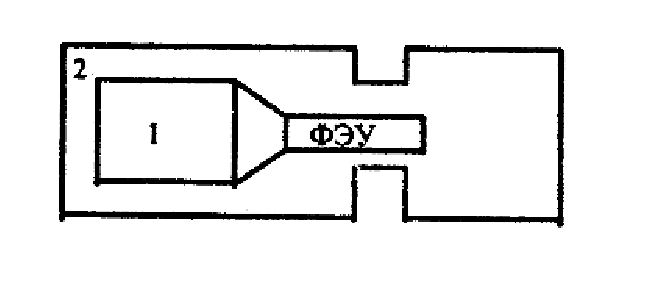
\includegraphics{Jelly.eps}
	\caption{Схема порогового счётчика Джелли} \label{Jelly-counter}
	\end{figure}

	Устройство (Pис.~\ref{Jelly-counter}) представляет из себя некоторый объём, заполненный радиатором, и фотоумножитель. Водный радиатор $ 1 $ находится в стеклянном контейнере $ 2 $ с посеребрёнными боковыми внутренними стенками. При отражении лучи попадают на ФЭУ, а серебрение помогает собирать черенковский свет с наименьшими потерями.
	
	Среди преимуществ пороговых счётчиков:
	\begin{itemize}
		\item простота устройства;
		\item высокая разрешающая способность во времени
	\end{itemize}
	
	\subsection{Дифференциальные черенковские счётчики}
	\label{sec:subsection}
	
	Если оптическая система детектора совершает фокусировку, детектор называется дифференциальным. Эти устройства предназначаются для измерения скорости частиц согласно выражению {\eqref{costheta}}.
	Происходит фокусировка света, идущего под углом $ \theta $ к направлению движения частицы на фотокатод ФЭУ. Задача дифференциального черенковского счётчика -- выбрать только те частицы, которые изучаются в эксперименте. 
	При пролёте через радиатор заряженной частицы среда излучает под одним и тем же углом во всех направлениях, в результате получается конус излучения.
	Чтобы зарегистрировать вспышки света, можно воспользоваться разными способами.
	
	 Радиатор детектора выбирается таким образом, чтобы сохранялось соотношение между углом излучения и направлением движения частицы, а также давал возможность этот угол $ \theta $ измерить.
	 \begin{figure}
	 	\noindent
	 	\hfil
	 	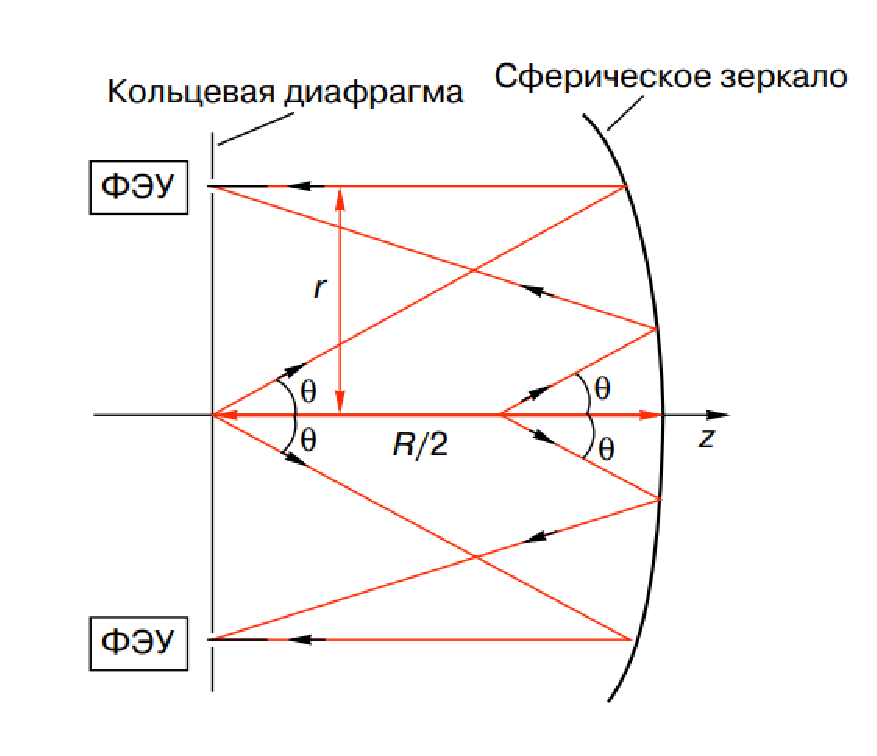
\includegraphics[height = 60mm]{Diffcounter.eps}
	 	\hfil
	 	\caption{Схема дифференциального черенковского счётчика с зеркалом}
	 	\label{diffscheme}
	 \end{figure}
	Таким требованиям вполне отвечает, например, радиатор в форме цилиндра. Пучок быстрых заряженных частиц влетает в основание \textit{параллельно} его оси.
	Они, в свою очередь, вызывают эффект Вавилова-Черенкова. Если выделяется определённый сорт с одинаковыми скоростями движения, свет будет выходить из торца радиатора под одинаковыми углами к оси, и с помощью оптической системы можно сфокусировать его на фотокатод. 
	Излучение от частиц, проходящих с другими скоростями, соответственно, проходит под иными углами, оно выходит из радиатора сходящимся или расходящимся пучком, и не будет попадать на ФЭУ.
	Из начального пучка заряженных частиц с разными скоростями будут зарегистрированы только частицы с относительной скоростью $\beta = 1/(n \cos{\theta}) $. Рассмотрим следующий способ эффективно разделись частицы по скоростям.
	
	\subsection{Счётчики типа RICH}
	\label{sec:subsection}
	Для частиц очень высоких энергий регистрация с помощью черенковских детекторов сопряжена с некоторыми трудностями.
	Во многих экспериментах на ускорителях изучаются взаимодействия высокоэнергичных пучков с мишенями из разных материалов.
	В результате таких столкновений образуется большое количество вторичных частиц, разлетающихся в широком диапазоне углов.
	Поэтому  эти частицы не могут быть зарегистрированы при использовании вышеописанных дифференциальных черенковских счётчиков.
	Для этого используются детекторы типа RICH (Ring Imaging CHerenkov counter). 
	В фокальной плоскости сферического зеркала устанавливаются детекторы, позволяющие определить радиус и положение центра кольца от сфокусированного зеркалом черенковского излучения. 
	Размеры колец напрямую связаны со скоростями частиц, вызвавших свет, а если известен ещё и импульс, несложно определить массу продукта реакции. 
	
	Излучающей средой в РИЧ-детекторах являются преимущественно газы или аэрогель – наилегчайший твердый прозрачный материал, успешно заменяющий громоздкие газовые радиаторы при пороговых скоростях частиц $\beta \leq 0.993$.
	
	Структуру аэрогеля образуют сферические кластеры из кварца диаметром $ \sim 4 $ нм, формирующие трёхмерную сетку, поры которой заполнены воздухом. 
	Расзмеры пор гораздо больше размеров кластеров и могут регулироваться при создании аэрогеля, позволяя при этом добиться коэффициента преломления $ 1,007 - 1,1 $.
	Будучи твердым веществом, аэрогель позволяет конструировать компактные черенковские детекторы, что особенно важно для применения их в исследованиях на космических аппаратах. 
	
	\subsection{Черенковские детекторы полного поглощения}
	\label{sec:subsection}
	
	Во многих задачах физики важно определять энергии нестабильных частиц, распадающихся через очень короткое время на электроны и $ \gamma $-кванты.
	Непосредственно их невозможно зарегистрировать.
	Изучение таких частиц возможно только при регистрации продуктов их распада.
	
	Основным способом регистрации высокоэнергичных (порядка нескольких ГэВ) электронов и $ \gamma $-квантов является метод полного поглощения создаваемых ими электромагнитных ливней.
	 Рассмотрим само явление возникновения и происхождение электромагнитных ливней. 
	В поле атомных ядер у электрона или позитрона начинается тормозное излучение $\gamma$-квантов: $$e + A \longrightarrow e' + \gamma + A',$$ где штрих над элементом означает изменение энергии частицы. 
	Другим возможным процессом является образование из $
	\gamma$-кванта электрон-позитронной пары.
	При этом у него должна быть энергия порядка десятков МэВ. $$\gamma + A \longrightarrow e^- + e^+ + A'.$$
	
	При попадании высокоэнергичного $ \gamma $-кванта в достаточно толстый слой вещества, размер которого превышает длину свободного пробега $ \gamma $-кванта до рождения электрон-позитронной пары (что составляет около 5 -- 10 мм для плотных сред) через короткое время частица превратится в $e^-e^+$-пару, которые, в свою очередь будут тормозить в среде. 
	Тормозные $\gamma$-кванты будут заново рождать пары и так будет лавинообразно продолжаться всё то время, пока реакции тормозного излучения и рождения электрон-позитронной пары доминируют (то есть для них достаточно энергии).
	\begin{figure}
		\noindent
		\hfil
		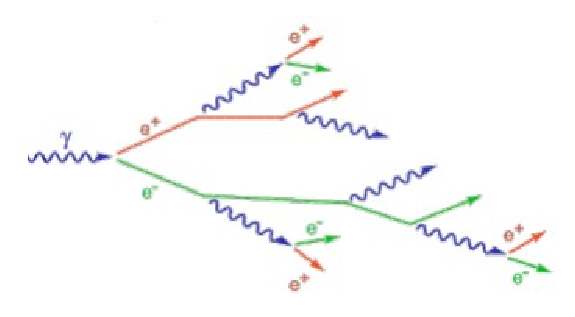
\includegraphics[height = 60mm]{elec.eps}
		\hfil
		\caption{Схема электромагнитного ливня.}
		\label{emrain}
	\end{figure}
	
	Схему такого электромагнитного ливня можно увидеть на (рис. \ref{emrain}).
	Энергия каждой дочерней частицы будет в среднем равна 1/4 энергии начальной.
	
	При малых энергиях решающую роль будут играть другие процессы вроде ионизационных потерь электронов и позитронов, из-за чего поток частиц уменьшится.
	Ливень также может возникнуть не только от $ \gamma $-кванта, но и от электрона или позитрона, и развиваться будет аналогично.
	
	Если вышеописанная реакция происходит в прозрачном веществе, то при обладании частицей необходимой скоростью в среде будет возникать черенковское излучение. 
	Если толщина вещества достаточна для полного поглощения ливневых частиц, число фотонов будет пропорционально энергии первичной частицы, вызвавшей ливень. 
	На этом основан принцип измерения энергии черенковскими спектрометрами полного поглощения. 
	В качестве их радиаторов используются очень прозрачные стёкла, а также некоторые кристаллы. 
	\subsection{Детекторы для регистрации космических лучей}
	\label{sec:subsection}
	
	В завершение этого раздела будет приведён ещё один тип черенковских детекторов.
	Его работа также основана на регистрации электромагнитных ливней, но теперь за их происхождение будут отвечать $ \gamma $-кванты с энергиями в несколько ТэВ ($ \sim10^{12}  $эВ), попадающие в земную атмосферу из космоса.
	Их источниками являются далёкие звёзды, и изучение спектров этих $ \gamma $-квантов поможет лучше понять процессы, происходящие во Вселенной.
	
	Черенковский свет регистрируется либо непосредственно ФЭУ, либо детекторами, похожими на прожекторы. 
	Необходимо уменьшить фон от постороннего света и определить движение первичного $ \gamma $-кванта.
	 Для облегчения задачи ставится несколько детекторов на небольшом расстоянии. 
	Событие регистрируется, если оно происходит одновременно на многих детекторах.
	Естественно, эксперимент ведётся только в безлунные ночи при прозрачной атмосфере. 
	
	Черенковское излучение сопровождает не только электромагнитные ливни, но и так называемые широкие атмосферные ливни (ШАЛ), возникающие от cильно взаимодействующих космических частиц (адронов). Для изучения ШАЛ также применяются черенковские детекторы.
	
	В качестве примера детектора для регистрации ШАЛ можно привести прототип черенковского телескопа для Якутской установки ШАЛ. Это широкоугольный телескоп с дифференциальными детекторами. 
	
	\section{Технические параметры черенковских детекторов}
	\label{sec:section}
	В данном разделе будут рассмотрены характеристики черенковских детекторов, разные качества пороговых и дифференциальных счётчиков, их разрешающие способности.
	
	\subsection{Временное разрешение}
	\label{sec:subsection}
	Конечная длительность светового импульса черенковского излучения, наблюдаемого на некотором расстоянии от траектории частицы, связана с зависимостью показателя преломления от длины волны (явление дисперсии). Наличие дисперсии приводит к некоторому размытию угла $ \theta $ черенковского излучения для частиц с данной скоростью $ v $. Так, для красного и фиолетового концов спектра, для которых показатели преломления соответственно $n_{\r}$ и $n_v$ черенковское излучение будет испускаться под углами 
	$$\theta_r = \arccos({1/\beta n_r}); \hspace{1.5cm} \theta_v = \arccos({1/\beta n_v})$$	
	
	Происходит размытие угла $\Delta\theta = \theta_v - \theta_r$. Оно приводит к существованию конечной длительности светового импульса для наблюдателя, находящегося на некотором расстоянии $l$ от траектории частицы. Длительность определяется временем, необходимым для прохождения <<фиолетовым>> фронтом расстояния, которое в поле зрения наблюдателя разделяет его с <<красным>> фронтом.
	Это время характеризуется формулой $\tau = \frac{1}{\beta n}(\tg{\theta_v} - \tg{\theta_r})$. При высоких показателях преломления и низкой дисперсии это величина $\tau \sim 10^{-12} c$.
	
	Временное разрешение черенковского детектора без фокусировки определяется временем нарастания светового импульса на фотокатоде ФЭУ и временными характеристиками самого ФЭУ. Время нарастания светового импульса на фотокатоде ФЭУ несколько больше длительности собственного светового импульса черенковского излучения ($10^{-12} - 10^{-11}$ с), так как черенковское излучение в детекторах без фокусировки прежде чем попасть на фотокатод, испытывает отражение от стенок радиатора. Поэтому время нарастания светового импульса на фотокатоде ФЭУ зависит от отражающих свойств стенок радиатора. В радиаторах с диффузным отражателем это время превышает длительность собственного черенковского излучения и составляет около $10^{-8} c$. При зеркальном отражении разрешающее время составляет $\sim 10^{-10}$ c для радиаторов небольших размеров (20 -- 30 см).
	
	Временное разрешение детекторов с фокусировкой определяется временными свойствами фотоумножителей, так как длительность черенковского излучения $10^{-11}$~--~$10^{-12}$ с, а ФЭУ обычно воспроизводят без искажения лишь световые сигналы длительностью $10^{-10}$~--~$10^{-9}$ с.
	\subsection{Энергетическое и скоростное разрешения}
	\label{sec:subsection}
	От свойств радиатора также зависит, в каком диапазоне скоростей частиц работает детектор. Продифференцировав соотношение \ref{costheta} можно получить:
	\begin{align}
	&		\Delta\beta / \beta = \tg{\theta}\Delta\theta = \sqrt{(n^2\beta^2 - 1)}\Delta\theta
	\label{velocity}
	\end{align}
	
	 Для разделения по скоростям частиц высоких энергий ($ \beta \rightarrow 1 $) используются газовые радиаторы с показателем преломления $ n \approx 1,01 $. Разрешение таких счётчиков составляет $\Delta\beta \approx 10^{-6}$. Угол излучения света близок к одному градусу.
	 
	 \section{Спектрометрия релятивистских электронов}
	 Черенковские детекторы применяются в спектрометрии электронов. Диапазон 1 -- 10 МэВ выбран неслучайно, это энергии, соответствующие релятивистским электронам, или т.н. электронам-убийцам (killer-electrons). 
	 Проникая через защитные корпусы космических аппаратов, они могут попадать прямиком в микросхему и приводить к неисправностям и даже к поломке аппаратуры. 
	 Черенковские детекторы для спектрометрии электронов использовались на космических аппаратах <<Галс>> от Института Прикладной Геофизики, было 5 блоков при запуске "ГЛОНАСС-М" в 2005 году.
	 В 2014 году был разработан и создан экспериментальный прототип широкоугольного черенковского телескопа для совместной работы со сцинтилляционными детекторами Якутской установки ШАЛ.
	 
	
\end{main}
	%\begin{Kur-Finish}
	\fontsize{16}{14pt}\selectfont
	\newpage
	
	\part{Заключение}
	\label{sec:part}
	Подводя итог работе, необходимо отчитаться о выполненных задачах среди поставленных. Также стоит отметить несколько нюансов. Итак, следующие этапы были пройдены:
	\begin{itemize}
		\item изучен эффект Вавилова-Черенкова, его история открытия, проявления в природе;
		\item составлен обзор различных типов детекторов черенковского излучения, а также задач, для выполнения которых эти детекторы применяются;
		\item дано качественное описание разрешений черенковских детекторов;
		\item приведены примеры использования счётчиков для спектрометрии релятивистских электронов.
	\end{itemize}
	
	Расчёт разрешений реальных детекторов вызвал некоторые трудности, в том числе и из-за отсутствия опытного образца. Вследствие этого работа является исключительно обзорной, однако вызвала у меня желание углублять знания в этом направлении.
	
	К сожалению, довольно долгое время черенковские детекторы почти не используются в спектрометрии релятивистских электронов. 
	Один из экспериментов по построению их спектра был проведён в Дубне в 1974 году и представлял собой одновременное использование черенковского детектора диапазона 3 -- 10 МэВ и полупроводникового детектора с диапазоном 0,5 -- 5 МэВ. Спектры получились одинаковой формы, но в области перекрытия диапазонов они никак не коррелировали. Виной тому могут быть неправильный учёт геометрического фактора установки или неисправности аппаратуры. Точного ответа на несоответствие экспериментальных данных не было дано. 
	
	 Глобальная задача, являющаяся не более, чем перспективным планом -- вернуть черенковские детекторы в спектрометрию электронов и использовать их на космических аппаратах.
	 В дальнейшем планируется изучить причины ухудшения углового разрешения счётчиков и способы их улучшения.
\end{Kur-Finish}% заключение
	%\documentclass{article}

\usepackage[utf8x]{inputenc}
\usepackage[english, russian]{babel}
\usepackage[T2A]{fontenc}
\usepackage{amsmath}

\begin{document}
	Шаблон текста
\end{document}% приложение
	\newpage
	
	\begin{thebibliography}{0}
		\bibitem{bolotovsky}Болотовский~С.М.
		Теория эффекта Вавилова-Черенкова. --- УФН 62 201–246 (1957)
		\bibitem{soros}	Денисов~С.П.
		Излучение <<сверхсветовых>> частиц (эффект Черенкова). --- Соросовский образовательный журнал, номер 2, 1996.
		\bibitem{podorozny} Д. М.~Подорожный, А. Н.~Турундаевский, В. Я.~Шестоперов. Изучение космических лучей высокой энергии с помощью черенковского излучения, рождённого заряженной частицей в верхних слоях атмосферы. --- Вестник Московского университета. Серия	3. Физика. Астрономия.	2001. н.6.
		\bibitem{akimov}Акимов~Ю.К.
		Черенковские детекторы в физике частиц. --- Ядерная физика, т.67, н.7, 2004
		\bibitem{prak}Специальный ядерный практикум.
		Черенковский детектор.
		\bibitem{yakushal}А.А.~Иванов, С.П.~Кнуренко, А.Д.~Красильников, И.В.~Ксенофонтов,
		З.Е.~Петров, М.И.~Правдин, Л.В.~Тимофеев, И.Е.~Слепцов.
		Разработка прототипа широкоугольного черенковского телескопа для якутской установки ШАЛ. --- Известия РАН. Серия физическая, 2014, т.78, н.3.
	\end{thebibliography}
\end{document}